\multiproblem{0}{
\begin{enumerate} 
\item{A configuration of a system is given in Figure \ref{fig:block1}. Given that the block has a mass m=10kg, and the coefficient of friction between the block and the surface is $\mu=1$:}
     \begin{itemize} 
        \item{What is the normal force on the block?\\ %\A $F_N=$Weight of block $=mg=98.1$N
        }
        \item{If an external horizontal force of 10N is applied to the block will it remain in equilibrium? %\A Yes: $F_f\leq\mu F_N=\mu m g =98.1$N$>10$N
        }
        \item{What is the maximum horizontal force that can be exerted upon the block without it moving? %\A $F_H=F_f\leq 98.1$N and so the maximum force is 98.1N
        }
        \item{Suppose we now do not know the value of the coefficient of friction $\mu$, but that the largest horizontal force we can exert upon the block without it moving is 32.7N. What is the new value for the coefficient of friction in this case? %\A As forces are balence in this equilibrium $F_H_{max}=F_f_{max}= \mu m g$. And so by rearranging $\mu=\frac{F_H}{mg}=\frac{1}{3}\approx 0.33$	
        } 
     \end{itemize}
\end{enumerate}
}


\multiproblem{1a}{
\begin{enumerate}
\item Figure  \ref{blahdiblah} shows a configuration of a mass which we will treat as a point particle hanging on a light spring. The particle has mass $m$, and the distance of the particle from the ceiling is $x$m. th spring has the following propeties: spring constant $k$N/m and natural length $l$.
\begin{itemize}
	\item{ Firstly, justify that the units of the spring constan are N/m with the use of Hooke's Law. %\A Force (N) = constant $\times$ extension (m), and so constant= Force (N) / extension (m)
	}
	\item{Find the distance $x$ given that $m=10$kg, $k=109$N/m and $l=$1m. %\A Restorative spring force $F_s=k(x-l)$, weight $F_G=mg$, forces balenced and so $F_s=F_G=k(x-l)=mg$, and so $x=\frac{mg}{k}+l=0.9+1=1.9$m
	}
	\item{Now instead, find a general expression for the distance $x$ in terms of the parameters $m,l,g,k$. %\A see above
	}
	\item{Sketch the distance $x$ as a function of $k$ (you can use $m=10$kg and $g=9.81$m/s$^2$) and label key features.%\A 
	}
\end{itemize}
\end{enumerate}
}

\multiproblem{1b}{
\begin{enumerate}
item Figure \ref{Blahdiblah} shows a configuration of a block of mass $m$kg on a surface. The block is also attached by a spring (with spring constant $k$N/m and natural length $l$) to the wall and the distance from this wall is given by $x$.Given that $m=1$ kg and $l=1$m:
\begin{itemize}
	\item{ What is the value of the normal reaction force on the block? %\A  Normal force and weight are balanced $F_n=mg=9.81$N
	}
	\item{Assuming that the surface is smooth ($\mu=1$) and the spring constant $k>0$, state the distance $x$ at which the system is in equilbrium. %\A The horizontal forces must balance so the spring force $F_s=k(x-l)$ is equivalent to the frictional force $F_f\leq\mu F_N$, since $\mu=0$ this frictional force must also equal 0 and so $F_s=k(x-l)=0$ which implies $x=l$m
	}
	\item{Assume now that the surface is rough and that the coefficient of friction $\mu=1$. Furthermore, the srping constant is known to be $k=30$N/m. What is the range of values of $x$ for which the block may be in equilibrium? %\A 1-0.327\leq x\leq 1+0.327.
	}
\end{itemize}
\end{enumerate}
}

\multiproblem{1c}{
\begin{enumerate}
\item{Figure \ref{fuckingfuck} shows a cofiguration of masses and pulleys. Both the block and the particle have mass $m=1$kg}
\begin{itemize}
	\item{Draw free body force diagrams for both the block and the particle}
	\item{Point b is at position $(-1$i$,1$j$)$ from point O. If $m=1$kg and $\mu=1$ can the system be in equilibrium? %\A Yes: If in equilbrium the forces are balancd on the particle and so the tension in the pulley string is equivalent to the weight of the particle ($T_p=mg$). Now looking at the block we can see that the frictional force must act on the block in the direction down the slope. So assuming equilbrium, resolving the forces parallel to the slope we have $T_p=mg=mg$sin$(\theta) + F_f$ where $theta$ is the angle of the slope. This angle of the slope with the horizontal can be found to be $theta=45^o=\pi/4$rad from the position vector. Furthermore, the frictional force is given by the inequality $F_f\leq \mu F_N$ where $F_N$ is the normal force (perpendicaular to the slope). This can be found to give $F_f\leq \mu  mg$cos$(\theta)$. If we substitute this into the earlier equation we find $mg(1-$sin$(\theta))=F_f\leq\mu  mg$cos$(\theta)$ which simplifies to $1-$sin$(\theta)\leq$cos$(\theta)$ which is easily shown to be true. 
	}
	\item{What is the critical value of $\mu$ (the smallest value such that the system may still be in equilbirum)? %\A At this critical point $F_f=\mu F_n$ and so it can be found in the same way as before that $\mu mg$cos$(\theta)+mg$sin$(\theta)=mg$ which can be easily rearranged to give $\mu=(1-$sin$(\theta))/$cos$(\theta))=\sqrt{2}-1\approx 0.41	$
	}
\end{itemize}
\end{enumerate}

}


\multiproblem{2}{Masses on slopes
\begin{enumerate}
\item Consider a mass $m$ on a slope at angle $\alpha$ to the horizontal. Assume the surface of the slope has a coefficient of friction $\mu$. 
            \begin{center}
                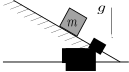
\includegraphics[scale=0.4]{fig_1.pdf}
            \end{center}
            \begin{enumerate}
            	\item Draw a free-body diagram of the system
		\item If mass $m = 10$ is located at point $(x,y) = (-2,1)$ and the slope makes contact with the horizontal ($x$-axis) at point $(0,0)$, determine the maximum value of the 			friction force, $F$, which ensures the system is in equilibrium. {\it Assume $\mu =1$}.
			%\A First find $\alpha$
		\item In the absence of friction, what would be the acceleration of the mass? 
		%\A Acceleration acts down the slope and is therefore the net force parallel to the slope divided by the mass: $F = ma \to a = \frac{F}{m}$: $a = g\sin(\alpha)$
		\item Derive an inequality in terms of parameter $\alpha$ that defines the range of values of $\mu$ for which this system will remain in equilibrium.
		%\A We need to use Coulomb Friction: $|F| \leq \mu N$.
		%\A From the free body diagram: $N= mg\cos(\alpha)$ ($1$), $F = mg\sin(\alpha)$ ($2$).
		%\A Using $2$ and Coulomb Friction, we have $|mg\sin(\alpha)| \leq N \mu$, therefore (using $1$ to eliminate $N$), $\mu \geq |\tan(\alpha)|$
             	\item Sketch the variation in the maximum value of $\mu$ as a function of angle $\alpha$ for the range $0 \leq \alpha \leq \pi/2$. Interpret your sketch for large $\alpha$ ($\alpha 			\to \pi/2$). 
            \end{enumerate}
            
\item Consider the system in question 1.b placed on a slope that makes an angle $\alpha$ to the horizontal, such that the central axis of the spring is parallel to the surface of the slope. Assume the surface of the slope has a coefficient of friction $\mu$.
            \begin{center}
                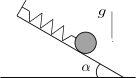
\includegraphics[scale=0.4]{fig_2.pdf}
            \end{center}
	\begin{enumerate}
		\item Draw a free body diagram of the system.
		\item Derive an inequality in terms of parameters $m$, $g$, $\alpha$, $k$, $L$ and $\mu$,  that defines the range of values of $x$, the length of the spring, for 					which this system is in equilibrium.
		%\A We need to use Coulomb Friction: $|F| \leq \mu N$, where $F$ is the net force acting parallel to the slope.
		%\A From the free body diagram: $N= mg\cos(\alpha)$ ($1$), $F = mg\sin(\alpha) - k(x-L)$ ($2$).
		%\A Using $2$ and Coulomb Friction, we have $|mg\sin(\alpha) - k(x-L)| \leq mg\cos(\alpha) \mu$
		%\A Rearranging: |x| \leq \frac{mg}{k}(\cos(\alpha) \mu - \sin(\alpha)) -L
		\item If the spring is replaced by one which is stiffer, how does this affect the range of extensions for which the mass is stationary? Use a sketch to demonstrate this result.
	\end{enumerate}
\end{enumerate}
}

\multiproblem{3}{Systems of 2 masses
\begin{enumerate}
\item 2 masses $m_1$ and $m_2$ are connected by a spring of stiffness $k_2$ and natural length $L_2$. Mass $m_1$ is also connected to a wall by a spring of stiffness $k_1$ and natural length $L_1$. The surface on which the masses are resting has a coefficient of friction $\mu$.
            \begin{center}
                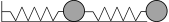
\includegraphics[scale=0.4]{fig_3.pdf}
            \end{center}
	\begin{enumerate}
	\item Draw a free body diagram for each mass.
	\item Find an expression for the range of values of $\mu$, the coefficient of friction, that ensure the system is in equilibrium. To simplify your expressions, use $\epsilon_i = x_i - L_i$ where $\epsilon_i$ corresponds to the extension of spring $i$.
	%\A From the free body diagrams we have: $N_1 = m_1g$, $N_2 = m_2g$, $F_2 = k_2(x_2-L_2) = k_2\epsilon_2$, $F_1 = k_1(x_1-L_1-x_2 + L_2) = k_2(\epsilon_1 - \epsilon_2)$
	%\A Applying Coulomb Friction to each mass we obtain: $|\frac{k_1}{m_1g}(\epsilon_1 - \epsilon_2) |\leq \mu$ and $|\frac{k_2}{m_2g}\epsilon_2| \leq \mu$
	%\A Summing the inequalities and dividing by $2$ gives: $|\frac{k_1}{2m_1g}(\epsilon_1 - \epsilon_2) +\frac{k_2}{2m_2g}\epsilon_2| \leq \mu$
	\item If $m_2 = \beta m_1$, $\epsilon_2 = \gamma \epsilon_1$ and $k_2 = \delta k_1$, using the expression from part ii, sketch a graph for $\mu$ as a function of $\beta$. Sketch another graph for $\mu$ as a function of $\delta$. How does this differ from a system of only one mass (question 1.b)?
	%\A Using the expression derived above and substituting for $m_2$, $k_2$ and $\epsilon_2$, we obtain:
	%\A $|\frac{k_1}{2m_1g}[\epsilon_1(1-\gamma +\frac{\delta \gamma}{\beta})| \leq \mu$
	\end{enumerate}


\item Two masses, $m_{1}$ and $m_{2}$ are connected by a spring with stiffness $k$ attached to a light inextensible string running smoothly over a pulley, as shown below.
            \begin{center}
                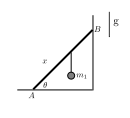
\includegraphics[scale=1.8]{fig_4.pdf}
            \end{center}
	    Mass $m_{2}$ rests on a slope at unknown angle $\theta$. 
            \begin{enumerate}
            \item Draw free body diagrams for both masses. Find the two horizontal and vertical force balance equations for each mass. 
	    \item Suppose $m_{1}$ and $m_{2}$ are known. If there is no friction acting on the slope, for which values of $\sin(\theta)$ is there a unique solution?
	    \item Now suppose there is friction, and that $m_{2}$, $\mu$ and $\theta$ are all known. What is the set of values of $m_{1}$ for which static equilibrium is possible? What is the corresponding extension of the spring,~$x$? Can $m_{1}=0$ and what is the condition in $\mu$ and $\theta$ for this to occur?  
	    %\A $m_2g = T$, $m_1g\cos(\theta) = N$, $T=k(x-L) - m_1g\sin(\theta)$
	    %\A $m_2g = k(x-L) - m_1g\sin(\theta)$
	    %\A $|F| \leq N\mu \to |m_2g - k(x-L)+ m_1g\sin(\theta)| \leq \mu m_1g\cos(\theta)$
	    %A  $- \mu m_1g\cos(\theta) \leq m_2g -k(x-L) + m_1g\sin(\theta) \leq \mu m_1g\cos(\theta)$
	    \end{enumerate}
 \end{enumerate}
}